
\subsection{State of art}

Process a large graph can be done via :
\begin{description}
    \item[New custom algorithm] implementation effort that mustbe repeated for each new algorithm
    \item[Distributed computing platform]  ill-suited for graph processing (map reduce)
    \item[Single-computer graph algorithm] doesn't scale
    \item[Parallel graph system] Not fault tolerant
\end{description}

\subsection{Pregel}
Pregel computations consist of a sequence of iterations, called supersteps.


During a superstep the framework invokes a userdefined function for each vertex, conceptually in parallel. 
The function specifies behavior at a single vertex V and a single superstep S.
Messages are typically sent along outgoing edges, but a message may be sent to any vertex whose identifier is known.

\subsection{Pregel model}

A typical Pregel computation consists of input, when the graph is initialized, followed by a sequence of supersteps separated by global synchronization points until the algorithm terminates, and finishing with output.

Algorithm termination is based on every vertex voting to halt. In superstep 0, every vertex is in the active state; all active vertices participate in the computation of any given superstep. A vertex deactivates itself by voting to halt. This means that the vertex has no further work to do unless triggered externally, and the Pregel framework will not execute that vertex in subsequent supersteps unless it receives a message. If reactivated by a message, a vertex must explicitly deactivate itself again. The algorithm as a whole terminates when all vertices are simultaneously inactive and there are no messages in transit.

% TODO : Improve this graph (need edges : message received, vote to halt)
\begin{figure}[!h]
    \centering
    \begin{tikzpicture}[node distance=2cm]
        \node[draw, circle] (Active) {Active node};
        \node[draw, circle, right=of Active ] (Inactive) {Inactive node};

        \draw (Active) edge[->](Active);
        \draw (Active) edge[ ->](Inactive);
        \draw (Inactive) edge[ ->](Inactive);
        \draw (Inactive) edge[ ->](Active);
    \end{tikzpicture}
    \\
    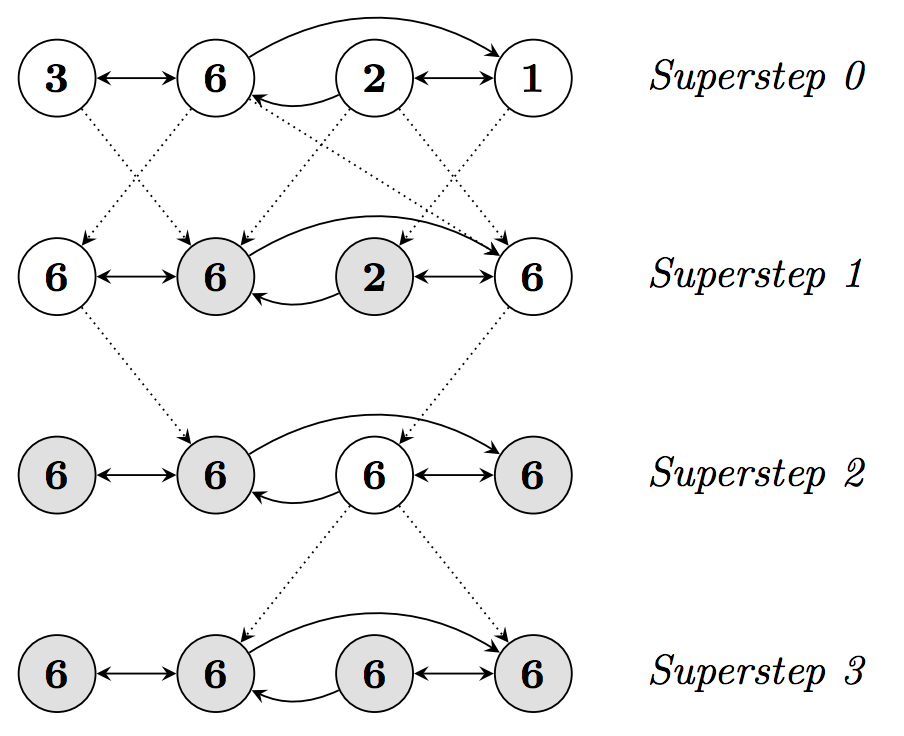
\includegraphics[width=0.5\linewidth]{img/pregelprop.png}
\end{figure}

\subsection{Pregel API}
\subsubsection{Message passing}
A vertex can send any number of messages in a superstep. All messages sent to vertex V in superstep S are available. There is no guaranteed order of messages in the iterator, but it is guaranteed that messages will be delivered and that they will not be duplicated.

A vertex could learn the identifier of a non-neighbor from a message received earlier.

\subsubsection{Combiners}
Sending a message, especially to a vertex on another machine, incurs some overhead. This can be reduced in some cases with help from the user.  For example, suppose that Compute() receives integer messages and that only the sum
matters, as opposed to the individual values. In that case the system can combine several messages intended for a vertex V into a single message containing their sum, reducing the number of messages that must be transmitted and buffered.


\subsubsection{Aggregators}
Pregel aggregators are a mechanism for global communication,
monitoring, and data. Each vertex can provide a value
to an aggregator in superstep S, the system combines those
values using a reduction operator, and the resulting value
is made available to all vertices in superstep S + 1.

For instance, a sum
aggregator applied to the out-degree of each vertex yields the
total number of edges in the graph.

\subsubsection{Topology Mutations}
Just as a user’s Compute() function can send messages, it can also
issue requests to add or remove vertices or edges.

Additions follow removals, with vertex
addition before edge addition, and all mutations precede
calls to Compute(). This partial ordering yields deterministic
results for most conflicts. (compute -> remove -> addition)

\subsubsection{Input and output}
Users with unusual needs can write their own
by subclassing the abstract base classes Reader and Writer.

\subsection{Architecture}
\subsubsection{Partition}
The default partitioning function is just hash(ID)
mod N, where N is the number of partitions, but users can
replace it.

\subsubsection{Processing}
\begin{itemize}
    \item Many copies of the user program begin executing on
        a cluster of machines. One of these copies acts as the
        master. It is not assigned any portion of the graph, but
        is responsible for coordinating worker activity. The
        workers use the cluster management system’s name
        service to discover the master’s location, and send registration
        messages to the master.
    \item The master determines how many partitions the graph
        will have, and assigns one or more partitions to each
        worker machine. The number may be controlled by
        the user. Having more than one partition per worker
        allows parallelism among the partitions and better load
        balancing, and will usually improve performance. Each
        worker is responsible for maintaining the state of its
        section of the graph, executing the user’s Compute()
        method on its vertices, and managing messages to and
        from other workers. Each worker is given the complete
        set of assignments for all workers.
    \item The master assigns a portion of the user’s input to
        each worker. The input is treated as a set of records,
        each of which contains an arbitrary number of vertices
        and edges. The division of inputs is orthogonal to the
        partitioning of the graph itself, and is typically based
        on file boundaries. If a worker loads a vertex that belongs
        to that worker’s section of the graph, the appropriate
        data structures (Section 4.3) are immediately
        updated. Otherwise the worker enqueues a message to
        the remote peer that owns the vertex. After the input
        has finished loading, all vertices are marked as active.
    \item The master instructs each worker to perform a superstep.
        The worker loops through its active vertices, using
        one thread for each partition. The worker calls
        Compute() for each active vertex, delivering messages
        that were sent in the previous superstep. Messages are
        sent asynchronously, to enable overlapping of computation
        and communication and batching, but are delivered
        before the end of the superstep. When the worker
        is finished it responds to the master, telling the master
        how many vertices will be active in the next superstep.
        This step is repeated as long as any vertices are active,
        or any messages are in transit
    \item After the computation halts, the master may instruct
        each worker to save its portion of the graph.
\end{itemize}

\subsubsection{Fault tolerance}
Fault tolerance is achieved through checkpointing. At the
beginning of a superstep, the master instructs the workers
to save the state of their partitions to persistent storage,
including vertex values, edge values, and incoming messages;
the master separately saves the aggregator values.

If a worker does not receive a ping message after a specified interval, the worker
process terminates. If the master does not hear back from
a worker, the master marks that worker process as failed.
When one or more workers fail, the current state of the
partitions assigned to these workers is lost. The master reassigns
graph partitions to the currently available set of workers,
and they all reload their partition state from the most
recent available checkpoint at the beginning of a superstep S. 


